\section{Resultados e discussões}
\subsection{Transformação genética de \textit{Escherichia coli} com proteínas
fluorescentes}
\begin{wrapfigure}[10]{l}{0.35\textwidth}
    \centering
    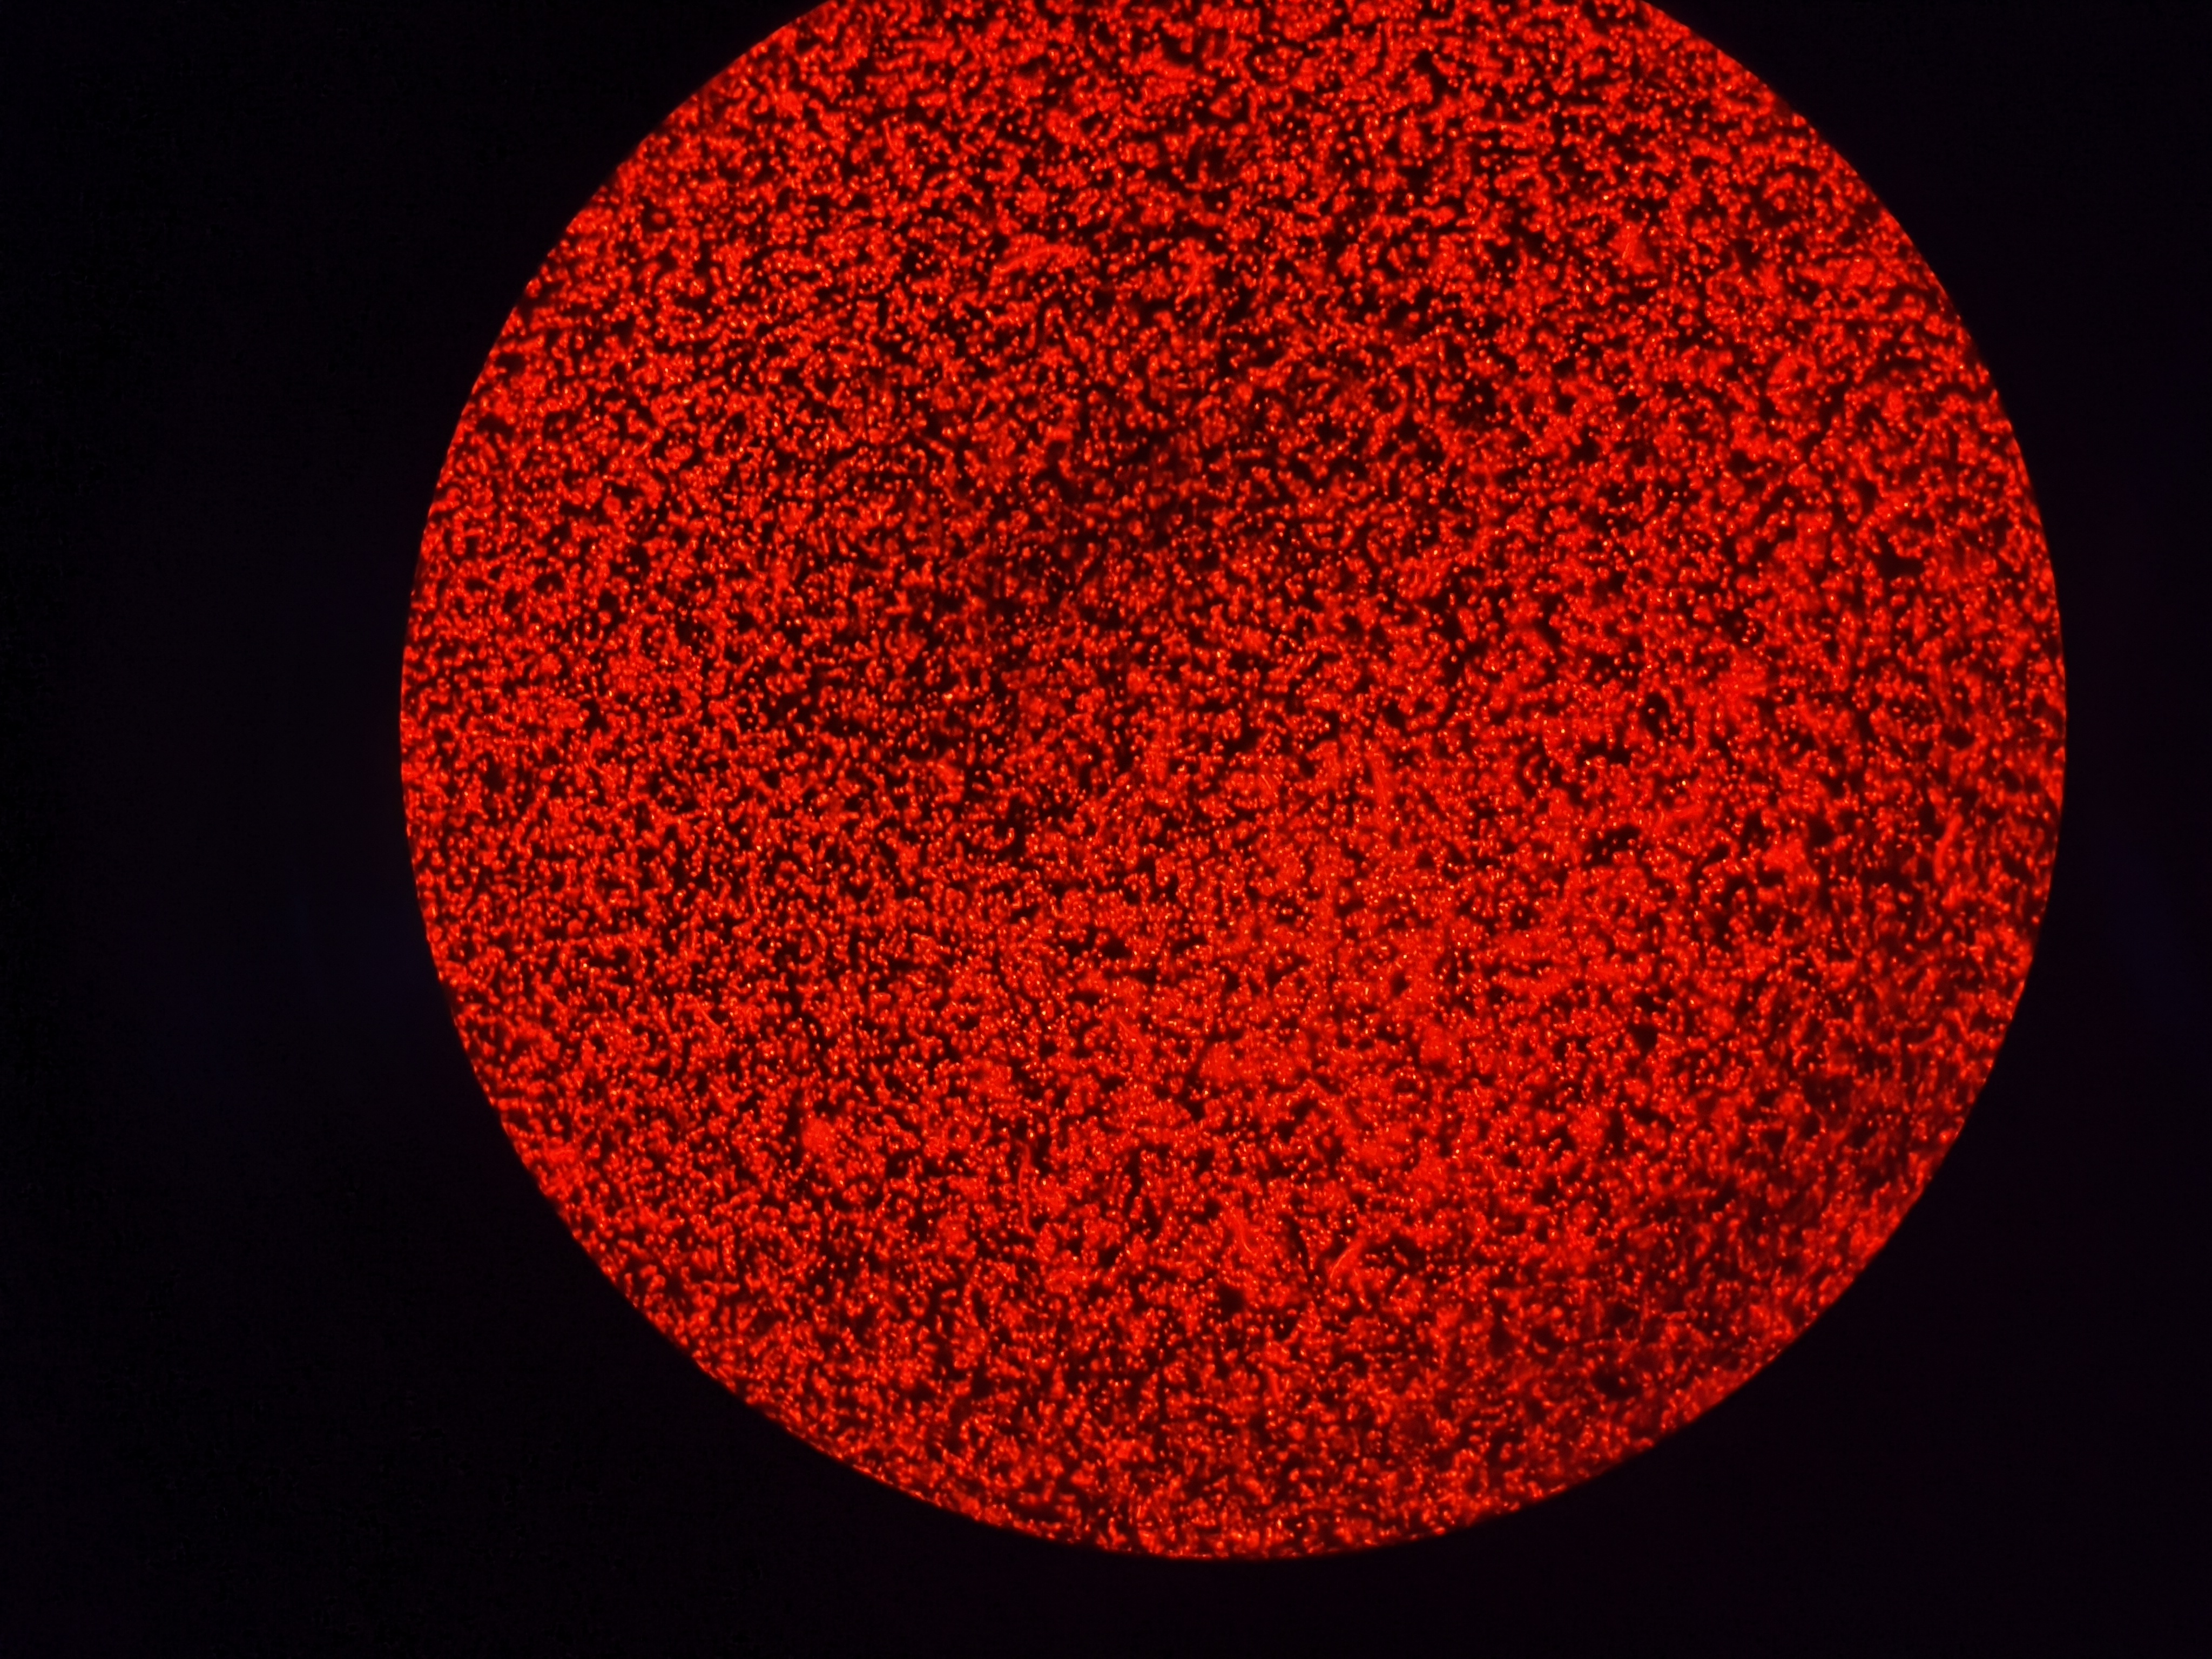
\includegraphics[width=.30\textwidth]{fig/red.jpg}
    \caption{Microscopia de fluorescência de \textit{Escherichia coli}
    transformada com plasmídeo contendo mCherry. Imagem retirada direto da lente
    ocular do microscópio.}
    \label{mCherry}
\end{wrapfigure}
Dentre os três plasmídeos testados, observou-se crescimento
bacteriano positivo em dois casos: (i) as colônias transformadas com o plasmídeo
contendo mCherry exibiram coloração vermelha característica, e (ii) as colônias
transformadas com mTAGbfp2 apresentaram fluorescência azul, conforme evidenciado
pelas imagens de microscopia de fluorescência. Veja a \cref{mCherry} e a
\cref{mTAG}.

\begin{wrapfigure}[10]{R}{0.35\textwidth}
    \centering
    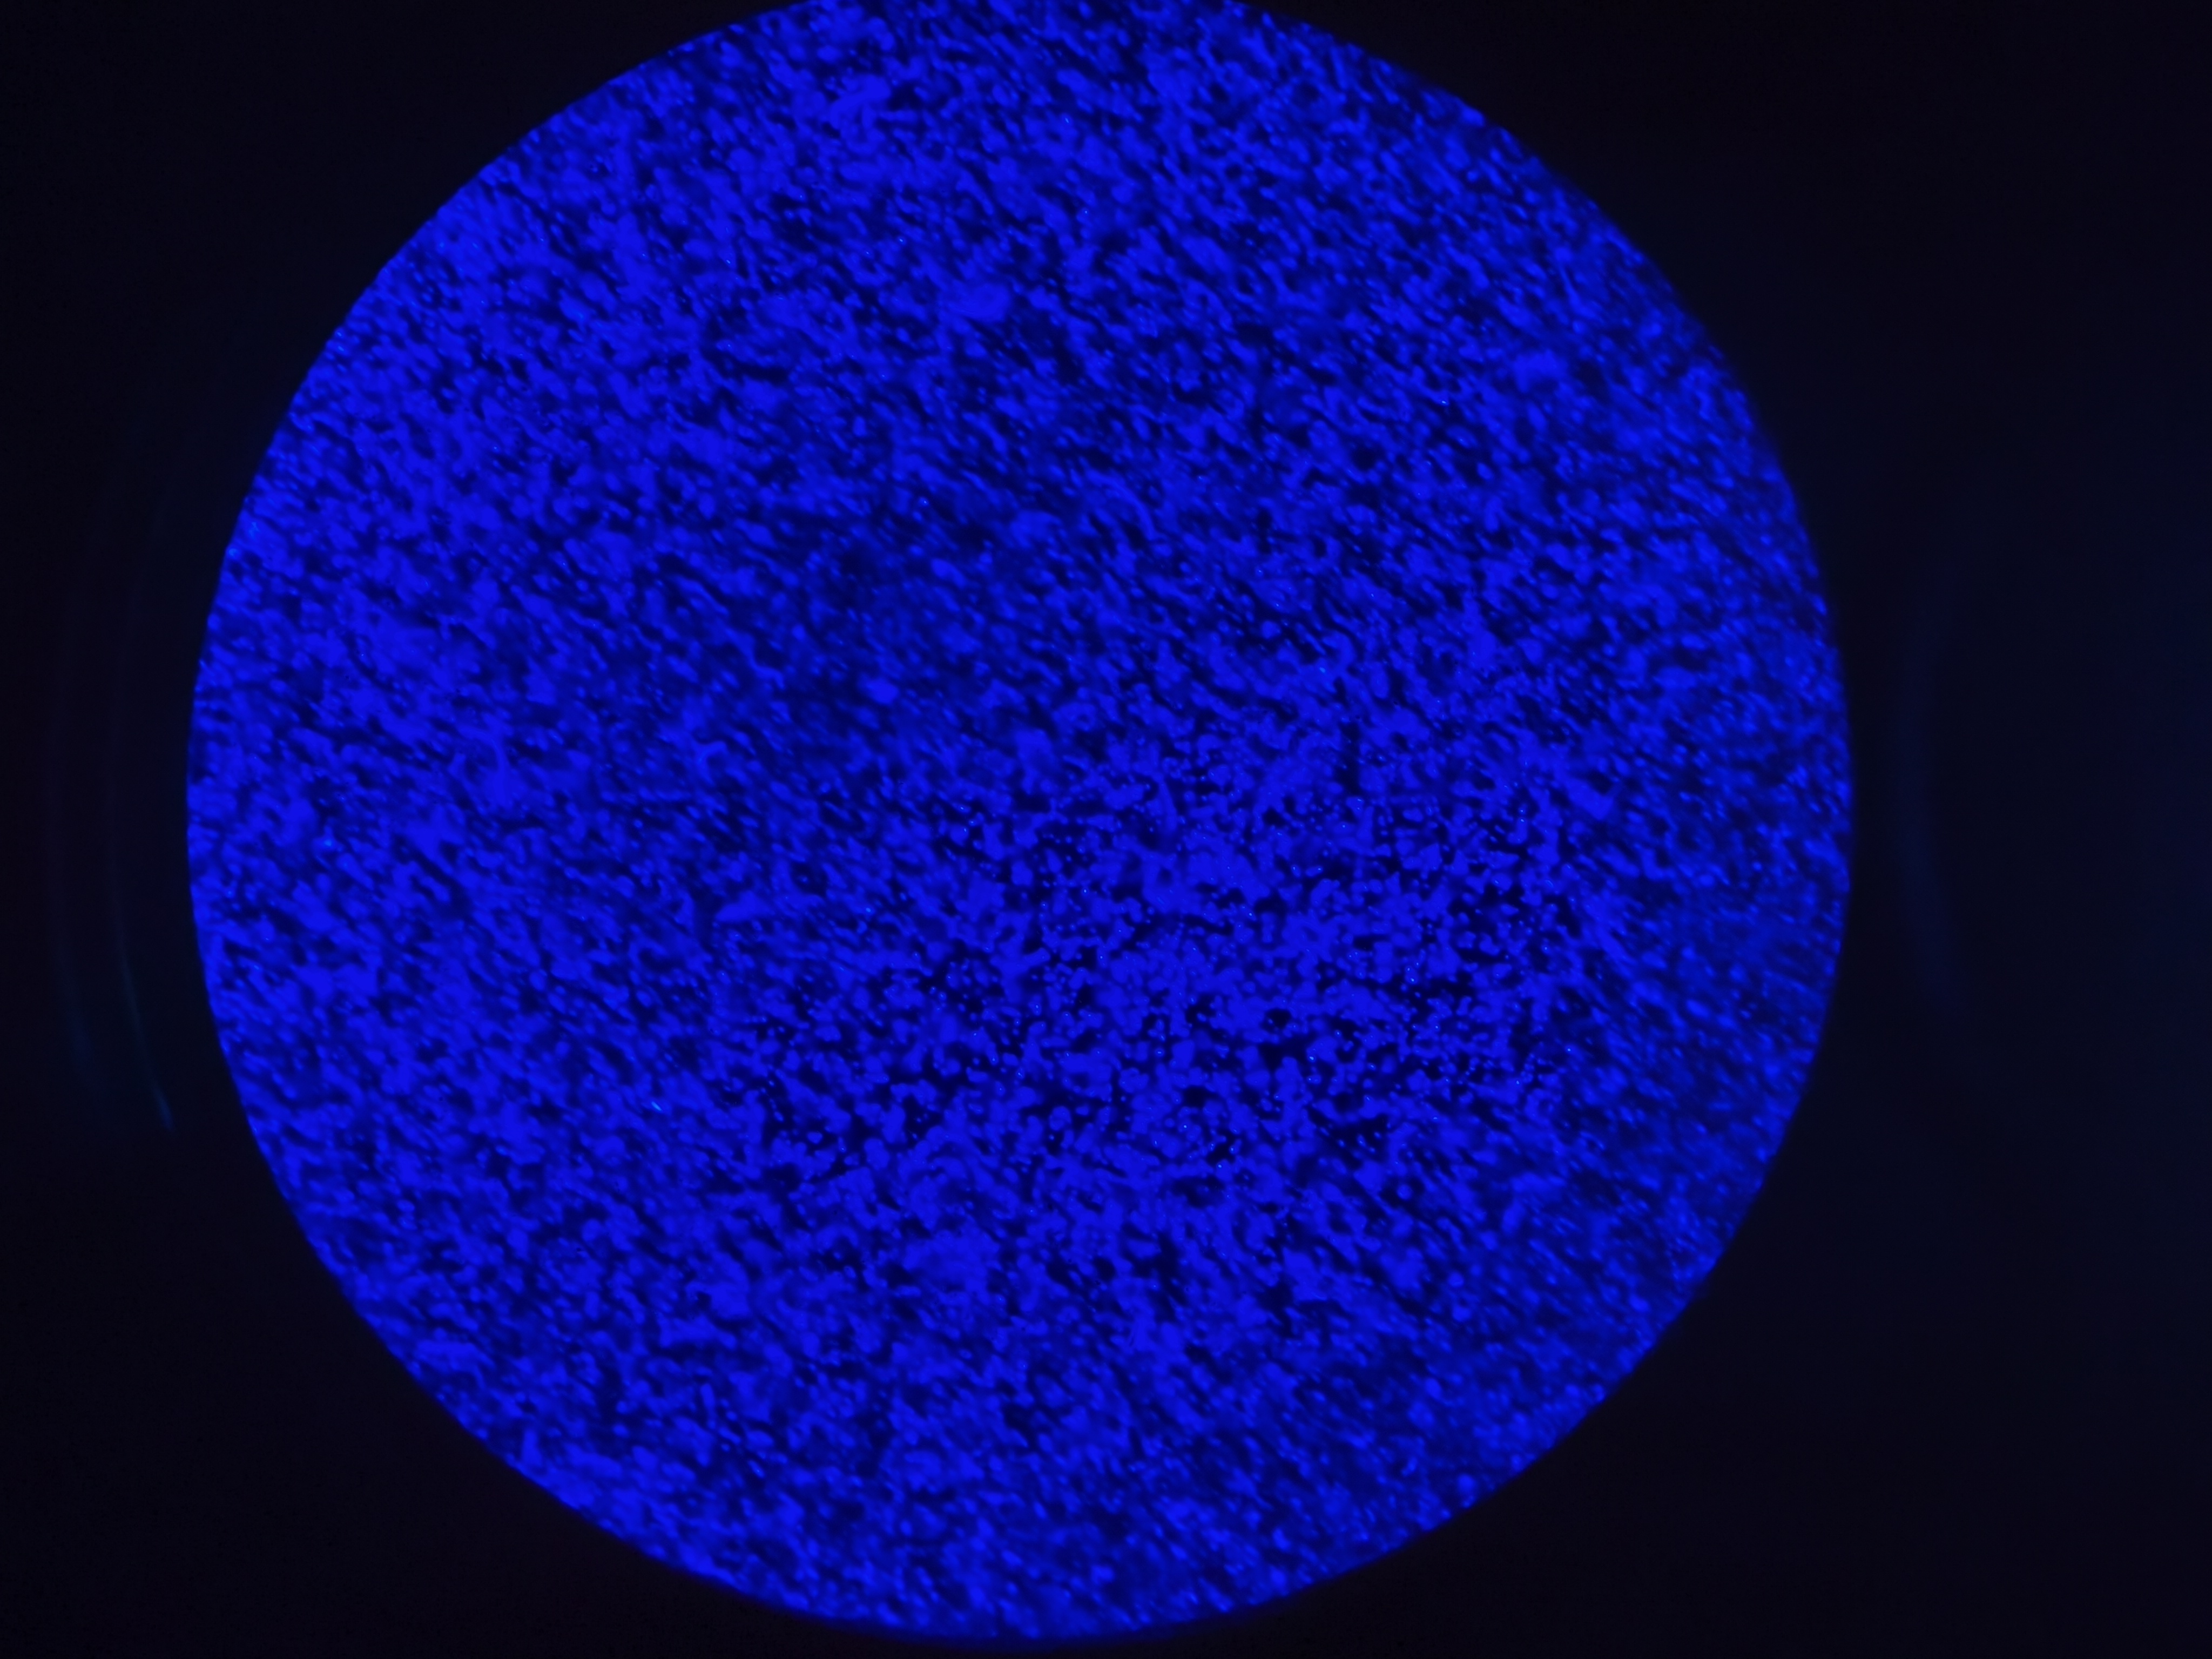
\includegraphics[width=.30\textwidth]{fig/blue.jpg}
    \caption{Microscopia de fluorescência de \textit{Escherichia coli}
    transformada com plasmídeo contendo mTAGbfp2. Imagem retirada direto da lente
    ocular do microscópio.}
    \label{mTAG}
\end{wrapfigure}

Em contraste, a transformação com o plasmídeo contendo GFP não resultou em
colônias viáveis, indicando falha nesse caso específico. Uma análise posterior
revelou que essa falha estava associada à baixa concentração do plasmídeo
durante a transformação, possivelmente devido à quantidade limitada disponível.
Esse fator técnico pode ter comprometido a eficiência da transformação,
explicando a ausência de crescimento bacteriano nessa condição.

Por fim, a correlação entre as cores observadas na transformações bem-sucedidas
e os marcadores genéticos esperados confirma a especificidade dos resultados
obtidos.

\subsection{Transformação genética de plantas por meio de Agroinfiltração
(\textit{Agrobacterium tumefaciens})}
Os procedimentos de transformação das plantas \textit{Nicotiana benthamiana},
\textit{Nicotiana tabacum} e \textit{Solanum lycopersicum} via
\textit{Agrobacterium spp.} foram executados conforme descrito nos métodos.
Porém, os resultados mostraram variação significativa na eficiência de
transformação entre as espécies, sendo observada expressão minimamente
significativas apenas na \textit{Solanum lycopersicum}. 

\begin{wrapfigure}[12]{R}{0.35\textwidth}
	\centering
	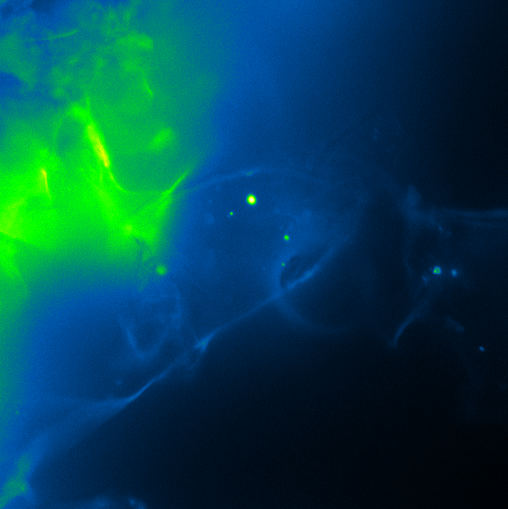
\includegraphics[width=.30\textwidth]{fig/tomate.png}
    \caption{Microscopia de fluorescência da secção transversal de
    \textit{Solanum lycopersicum}, transformada com plasmídeo contendo genes de
    expressão de GFP de localização nuclear. Imagem obtida por meio de microscopia
    de fluorescência e tratada com o programa ImageJ com adição de filtro Green Fire
    Blue}
	\label{lyco}
\end{wrapfigure}

Nas \textit{N.benthamiana} e \textit{N. tabacum}, a fluorescência associada á expressão do
transgene não foi detectada de forma alguma. Já na \textit{S.  lycopersicum},
embora a expressão também não tenha sido extremamente significativa, foi
possível observar regiões com fluorescência pontuais como mostrado na
\cref{lyco}, indicando uma resposta mais eficiente à agroinfiltração.

Essa diferença na eficiência da transformação e, principalmente, a completa
falta de expressão nas espécies de \textit{Nicotiana}, podem estar relacionadas a
diversos fatores, como a escolha errônea da área seccionada e sua orientação e o
tempo reduzido entre a agroinfiltração e a realização dos cortes, apenas dois
dias ao invés de cinco dias. Além disso, a ausência de observação de infecção pode indicar uma maior resistência à infecção
por \textit{Agrobacterium} nas espécies de \textit{Nicotiniana}.

